\section[Technische Funktionsweise von Bitcoin]{Technische Funktionsweise von Bitcoin\footnote{Dieser Abschnitt basiert auf \cite{nielsen}.}}
\label{sec:mechanics}

Mithilfe dieser kryptografischen Mechanismen lässt sich ein Zahlungsnetzwerk aufbauen, in welchem --~im Gegensatz zu herkömmlichen Banken~-- keine zentrale vertrauenswürdige Stelle notwendig ist.
Wie sich der Stand eines Kontos aus vorangegangen Transaktionen ergibt, so setzt sich auch der Kontostand einer Bitcoinadresse aus vorhergegangen Transaktionen zusammen.
Da es keine zentrale Stelle gibt, müssen alle Kontobewegungen und Guthabensstände öffentlich gemacht werden, um Betrug zu verhindern.

\subsection{Transaktionen}

\begin{figure}
    \begin{center}
		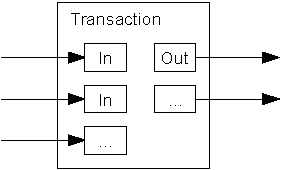
\includegraphics{transaction}
    	\caption{Transaktion aus Aus- und Eingängen \parencite[5]{nakamoto}}
    	\label{fig:transaction}
    \end{center}
\end{figure}

Transaktionen sind wohl der wichtigste Bestandteil des Bitcoin-Netzwerks.
Schon im White Paper zu Bitcoin werden Bitcoins als Kette von signierten Transaktionen definiert:

\begin{longquote}[2]{nakamoto}
We define an electronic coin as a chain of digital signatures. Each owner transfers the coin to the next by digitally signing a hash of the previous transaction and the public key of the next owner and adding these to the end of the coin. A payee can verify the signatures to verify the chain of ownership.
\end{longquote}

Denn anstatt einen Kontostand zu speichern und ihn bei jeder Transaktion zu verändern (was anfällig für Manipulation wäre), beziehen sich Transaktion auf vorhergegangene Transaktionen, damit die Herkunft und somit die Gültigkeit verifiziert werden.
Um Bitcoin zu versendenden, muss man also eine vorhergegangene Transaktion referenzieren, durch welche man die Bitcoins erhalten hat und anschließend die Transaktion signieren, um zu Beweisen, dass man jene besitzt.
Abbildung \ref{fig:transactionchain} zeigt eine Darstellung einer so entstehenden Transaktionskette, in der Bitcoins von Besitzer 0 bis zu Besitzer 3 wandern.

Da man aber nicht immer den vollen Betrag einer vorherigen Transaktion ausgeben möchte, muss es die Möglichkeit geben nur einen Teil der Bitcoins einer vorherigen Transaktion weiterzuschicken.
Ebenfalls sollte es möglich sein, zwei Transaktionen zu referenzieren und die Summe ihrer Bitcoins zu transferieren.
Um das zu ermöglichen, kann eine Transaktion, wie in Abbildung \ref{fig:transaction} dargestellt, aus mehreren Eingängen und mehreren Ausgängen bestehen.
Ein Eingang referenziert dabei immer einen Ausgang einer vorherigen Transaktion, welcher dabei unbrauchbar wird.%
\footnote{Möchte man nur einen Teil der Bitcoins aus der alten Transaktion ausgeben, so muss es zwei Ausgänge geben, wobei einer einen Teil an eine andere Adresse sendet und der andere den Rest wider zurück an einen selbst.}
Die Summe der Ausgänge ist dabei für gewöhnlich kleiner als die der Eingänge, da die Differenz als Transaktionsgebühr dient. (Siehe Abschnitt \ref{subsec:mining})

Nach dem Signieren der Transaktion wird diese von dem Bitcoin-Client über das Internet an andere Instanzen der Bitcoin-Software gesendet, welche die Transaktion auf gültigkeit überprüft und danach wiederum weitersendet.
So wird die Transaktion innerhalb kürzester Zeit mehrmals verifiziert und im gesamten Bitcoin-Netzwerk verteilt.

\subsection{Adressen}

\begin{figure}
    \begin{center}
        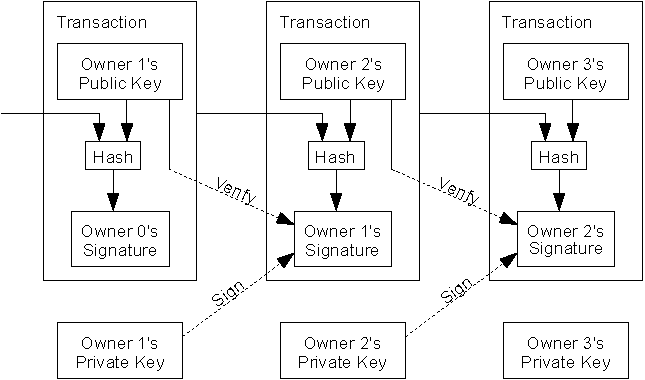
\includegraphics{transactionchain}
    	\caption{Unverzweigte Transaktionskette \parencite[2]{nakamoto}}
    	\label{fig:transactionchain}
    \end{center}
\end{figure}

Zum Signieren und Verifizieren von Transaktionen wird ein asymetrisches Schlüsselpaar benötigt.
Dadurch wird gewährleistet, dass nur autorisierte Personen die Ausgänge vergangener Transaktionen als Eingang in ihrer Transaktion verwenden können.
Erstellt man eine Transaktion, so referenziert man im Ausgang den öffentlichen Schlüssel des Empfängers der Bitcoin.
Möchte dieser die Bitcoin nun weitergeben so muss er diesen Ausgang in dem Eingang seiner Transaktion referenzieren.
Anschließend bildet er den Hashwert der Transaktion und signiert diesen mit seinem privaten Schlüssel.
Somit ist von jedem nachvollziehbar, dass es sich beim Ersteller der Transaktion um den Inhaber der Bitcoins handelt, indem man die Signatur mit dem öffentlichen Schlüssel aus der vorhergegangen Transaktion überprüft.

In Abblidung \ref{fig:transactionchain} werden diese Signaturen schematisch dargestellt.
Betrachtet man die mittlere Transaktion, in welcher Besitzer 1 seine Bitcoins an Besitzer 2 weitergibt, sieht man den Aufbau der Transaktions bestehnd aus dem öffentlichen Schlüssel des Empfängers, einem Hash aus diesem und der vorhergegangen Transaktion sowie der Signatur des Besitzers 1.
Diese Transaktion kann nun von jedem überprüft werden, indem er die Signatur mit dem öffentlichen Schlüssel aus der vorhergegangenen Transaktion verifiziert.

Diese öffentliche Nachvollziehbarkeit ist der Schlüssel in der Funktionsweise von Bitcoin.
Erst durch die aus der asymmetrischen Verschlüsselung folgenden Signaturen ist es möglich den Urheber einer Transaktion ohne eine zentrale Vertrauensstelle zu überprüfen.

Aufgrund der Tatsache, dass man nur den öffentlichen Schlüssel einer anderen Person braucht, um ihr Bitcoins zukommen zu lassen, wird dieser Bitcoin-Adresse genannt.
Die Bitcoinadresse ist eine 160~Bit lange Zahl, welcher eine 32~Bit lange Prüfsumme folgt.
Um die Handhabung zu vereinfachen wird diese Adresse mithilfe von Base58%
\footnote{\emph{Base58} ist analog zum Dezimal- oder Binärsystem ein Zahlensystem mit der Basis 58, das zur Darstellung der Zahlen neben Ziffern auch Buchstaben verwendet, wobei "`0"', "`O"', "`I"' und "`l"' aufgrund der Verwechsungsgefahr weggelassen werden.}
in 27-34 alphanumerische Zeichen kodiert.%
\footnote{Eine Bitcoinadresse sieht beispielsweise so aus: \texttt{1JQW4iRksV11pKSF4bnSXzeNMaqvc37Mq7}}

\subsection{Die Blockchain}

Um die Transaktion zu speichern werden alle Transaktionen, welche in einem bestimmten Zeitinterval stattfinden, in sogenannte \emph{Blocks} zusammengefasst.
Da jeder Block neben den Transaktionen auch eine Referenz in Form des Hashes auf den vorherigen Block beinhaltet, entsteht eine einzige lineare Kette von Blöcken -- \emph{Blockchain} genannt.
Aufgrund der Linearität der Blockchain kann gewährleistet werden, dass jeder Transaktions-Ausgang nur einmal von einem Eingang aufgegriffen wird und somit sogenannten \emph{Double-Spending} (d.\,h. das zwei- oder mehrmalige Verwenden eines Ausganges in verschiedenen Transaktionen) verhindert wird.

\subsubsection{Mining}
\label{subsec:mining}

Unter \emph{Mining} versteht man das Generieren von Blöcken.
Da man möchte, dass Blöcke nur so langsam erschaffen werden, dass sich das Bitcoin-Netzwerk über einen gemeinsamen aktuellen Block einig ist, ist ein gewisser Aufwand mit der Erstellungen eines Blockes verbunden.
Diese \emph{Proof-of-Work}-Mechanismen sorgen dafür, dass durchschnittlich nur alle 10 Minuten ein neuer Block erzeugt wird.

\begin{figure}
    \begin{center}
        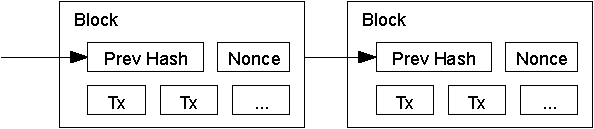
\includegraphics{blockchain}
        \caption{Vereinfachte Darstellung der Blockchain \parencite[3]{nakamoto}}
        \label{fig:blockchain}
    \end{center}
\end{figure}

Hierzu nimmt eine \emph{Mining-Software} die aus dem Bitcoin-Netzwerk empfangenen Transaktionen, welche noch nicht in der Blockchain vorhanden sind.
Darauf erstellt sie einen Block aus diesen Transaktionen und dem Hash des vorherigen Blocks.
(Siehe Abbildung \ref{fig:blockchain})
Dann berechnet sie den Hashwert des Blockes und vergleicht ihn mit dem Ziel-Wert.
Ist der Hash kleiner als der Zielwert, handelt es sich um einen gültigen Block.
Sollte der Hash größer sein, so gibt es einen 32-Bit großen Teil des Blockes (\emph{Nonce} genannt), welcher nach Belieben verändert werden kann, um einen entsprechenden Hash zu erhalten.
Da sich der Hash scheinbar zufällig ändert, muss der Miner relativ viele Hashwerte berechnen, bis er einen gültigen findet.
Der Zielwert wird anhand einer Formel alle zwei Wochen angepasst, damit egal wie viel Mining betrieben wird, immer durchschnittlich alle 10 Minuten ein gültiger Block gefunden wird.

Um die Miner für die aufgewandte Rechenleistung und Stromkosten zu entschädigen, verdient er auf zwei verschiedene Arten Bitcoin:
\begin{enumerate}
    \item Transaktionen beinhalten eine Transaktionsgebühr in Form einer Differenz zwischen Eingang und Ausgang.
    Ein Miner darf diese Transaktionsgebühr aus allen in seinem Block inkludierten Transaktionen an seine eigene Bitcoinadresse senden.
    \item Um Bitcoins zu erschaffen und einen Anfang für Transaktionsketten zu bieten, beinhaltet jeder Block eine Transaktion die Bitcoins aus dem Nichts schafft.
    Diese Belohnung für das Mining betrug am Anfang 50 Bitcoins pro Block, wird aber alle 210000 Blöcke (ca. alle 4 Jahre) halbiert, so dass Bitcoin trotz dauerhafter Zufuhr auf ein Maximum von 21 Millionen Bitcoins limitiert ist.
\end{enumerate}

Aufgrund dieser Eigenschaften kann Mining profitabel sein, wenn der Wert der erhaltenen Bitcoins über dem der Anschaffungs- und Betriebskosten der Mining-Hardware liegt.
Während es in den Anfängen von Bitcoin profitabel war, mit herkömmlichen Prozessoren Mining zu betreiben, welche zirka einige Millionen Hashwerte pro Sekunde berechnen können wurde bald durch die hohe Anzahl der Miner der Zielwert niedriger und es somit nicht mehr profitabel.
Da Grafikkarten für manche Rechenoperationen schneller sind als Prozessoren wurden darauf diese verwendet, womit fast eine Milliarde Berechnungen pro Sekunde möglich wurden.
Seit Ende 2012 gibt es auch dezidierte Mining-Hardware, welche nur dazu gebaut wird, Bitcoin-Mining zu betreiben.
Mit dieser Hardware sind inzwischen Geschwindigkeiten von bis zu 8~THash/s (8~Billionen Hashwertberechnungen pro Sekunde) möglich.

\subsubsection{Linearität}

Sollte es einmal vorkommen, dass ein Miner einen Block findet, bevor er den aktuellsten Block vom Bitcoin-Netzwerk erhalten hat, kommt es zu einer Verzweigung der Blockchain.
Hierbei kann es vorkommen, dass dieselben Bitcoins in jedem der Blöcke an verschiedene Empfänger gesendet werden.
Um zu verhindern, dass man somit Bitcoins verdoppeln kann, darf nur einer der zwei gleichzeitig generierten Blöcke weiterverwendet werden, während der andere für ungültig erklärt wird.
Die Auswahl des ungültigen Blocks geschieht gewissermaßen durch Zufall.
Während jeder Bitcoin-Client und jeder Miner zuerst den Block verwendet, den er als erstes erhalten hat, werden sich alle Beteiligten über einen Block einig, sobald ein Miner den nächsten Block findet, egal, welcher der beiden Blöcke als Ursprung dient.
Die in dem jetzt ungültigen Block gelisteten Transaktionen sind somit noch nicht verifiziert worden und werden in die nächsten Blöcke aufgenommen.
